\documentclass[aspectratio=169, 12pt]{beamer}

\usepackage[utf8]{inputenc}
\usepackage[T1]{fontenc}
\usepackage[catalan]{babel}
\usepackage{lmodern}
\usepackage{amsmath,amssymb}
\usepackage{mathtools}
\usepackage{xcolor}
\usepackage{graphicx}
\usepackage{bm}

\uselanguage{Catalan}
\languagepath{Catalan}
\usetheme{Frankfurt}
\useoutertheme{infolines}
\useinnertheme{rounded}
\usecolortheme{orchid}
\setbeamertemplate{navigation symbols}{}
\setbeamertemplate{footline}{}
\setbeamerfont{frametitle}{series = \bf}
\setbeamerfont{title}{series = \bf}
\setbeamerfont{headline}{series = \bf}

\AtBeginSection[]{
  \begin{frame}[plain]
  \vfill
  \centering
  \begin{beamercolorbox}[sep=8pt,center,shadow=true,rounded=true]{title}
    \usebeamerfont{title}\insertsectionhead\par%
  \end{beamercolorbox}
  \vfill
  \end{frame}
}

\let\P\relax
\DeclareMathOperator{\P}{P}
\DeclareMathSymbol{,}{\mathpunct}{operators}{"2C}
\renewcommand{\vec}[1]{\mathbf{\bm #1}}
\DeclareMathOperator{\gr}{gr}
\newcommand{\R}{\mathbb{R}}
\newcommand{\Z}{\mathbb{Z}}
\newcommand{\abs}[1]{\left\lvert #1 \right\rvert}

\title{Passejos aleatoris en grafs}
\author{Gerard Castro, Kim López, Ga\l.la Mora, Arnau Mas}
\date{5 de desembre de 2018}


\begin{document}
\begin{frame}[plain]
	\titlepage
\end{frame}


\begin{frame}
	\frametitle{Esquema}
	\centering
	\tableofcontents

\end{frame}

\section{Introducció}

\begin{frame}
	\frametitle{Definició}
	\begin{block}{Definició}
		Un \emph{passeig aleatori} a un graf \( G \) és una seqüència de vèrtexs \( v_1, v_2, \cdots, v_n, \cdots \), tal que \( v_kv_{k+1} \) es tria uniformement d'entre les arestes incidents a \( v_k \).
	\end{block}
\end{frame}

\begin{frame}
	\frametitle{Aspectes probabilístics}
	\( V(t) \) és la variable aleatòria que representa la posició del passeig a l'instant \( t \) \pause

	Les probabilitats de transició \[ \P(V(t) = u \mid V(t - 1) = v) \] determinen el passeig: \pause
	\begin{equation*}
		\P(V(t) = u) = \sum_{v \in V(G)} \P(V(t) = u \mid V(t - 1) = v) \, \P(V(t - 1) = v).
	\end{equation*}
\end{frame}

\begin{frame}
	\frametitle{Probabilitats de transició}
	Com que \[ \P(V(t) = u \mid V(t - 1) = v) = \frac{a(u,v)}{\gr(v)}, \] \pause
	tenim
	\[ P(V(t) = u) = \sum_{v \in V(G)} \frac{a(u,v)}{\gr(v)}P(V(t - 1) = v). \]
\end{frame}

\begin{frame}
	\frametitle{Un exemple}
	\begin{columns}
		\begin{column}{0.5\textwidth}
			\only<2>{
				\[ \P(V(0) = i_1) = 1 \]
			}
			\only<3>{
				\begin{align*}
					\P(V(1) = i_2) & = \P(V(1) = i_3) \\
												 & = \P(V(1) = i_4) = \frac{1}{3}
				\end{align*}
			}
			\only<4>{
				\[ \P(V(3) = i_1) = 1 \]
			}
		\end{column}

		\begin{column}{0.5\textwidth}
			\centering
			\only<2,4>{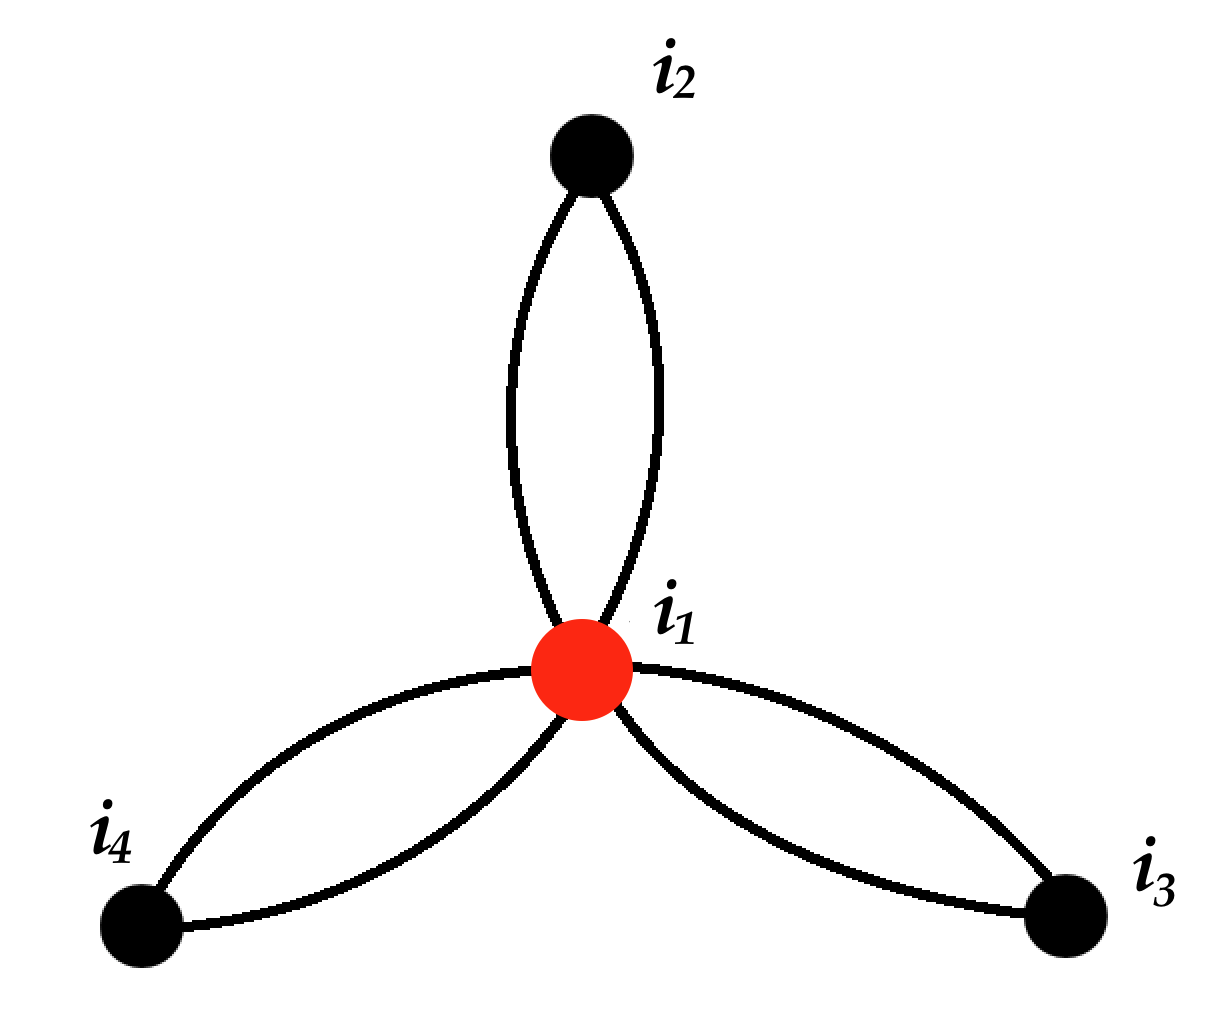
\includegraphics[scale = 0.15]{exemple-1.png}}
			\only<3>{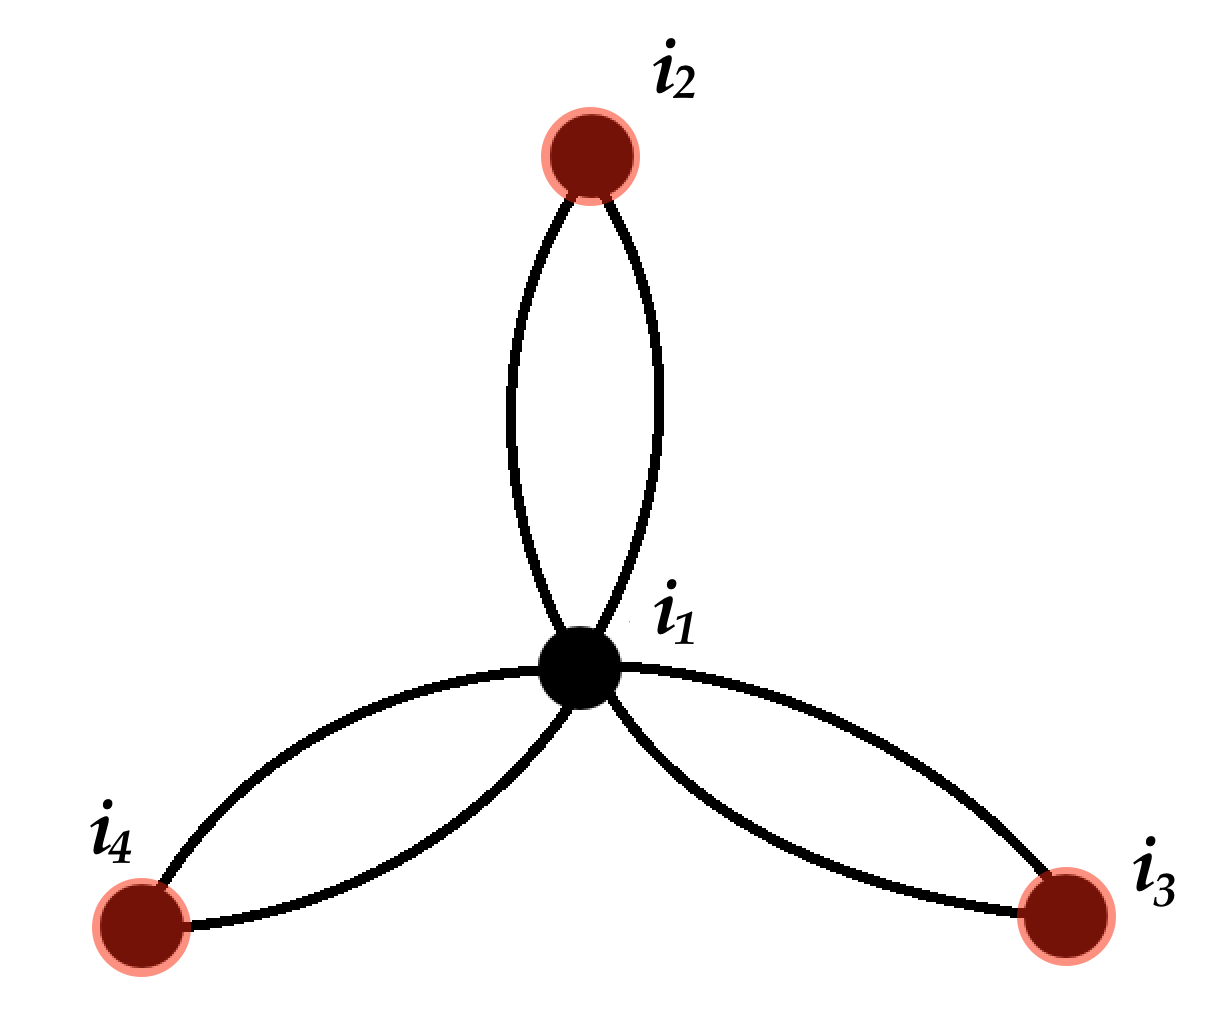
\includegraphics[scale = 0.15]{exemple-2.png}}

		\end{column}
	\end{columns}

\end{frame}

\begin{frame}
	\frametitle{Matriu de transició}
	Definim \( \vec{p}_t \in \R^{V(G)} \) com \( \vec{p}_t(u) = P(V(t) = u) \). \pause Aleshores, en forma matricial \[ \vec{p}_t = AD^{-1} \vec{p}_{t - 1}. \] \( A \) és la matriu d'adjacència i \( D \) la matriu dels graus. \( P = AD^{-1} \) és la \emph{matriu de transició}. \pause

	Per tant \[ \vec{p}_t = P^t \vec{p}_0. \]
\end{frame}

\begin{frame}
	\frametitle{Un exemple}
	\begin{columns}
		\begin{column}{0.5\textwidth}
			\only<2>{
				\begin{equation*}
					A = \begin{pmatrix}
						0 & 2 & 2 & 2 \\
						2 & 0 & 0 & 0 \\
						2 & 0 & 0 & 0 \\
						2 & 0 & 0 & 0
					\end{pmatrix} 
					\, D = \begin{pmatrix}
						6 & 0 & 0 & 0 \\
						0 & 2 & 0 & 0 \\
						0 & 0 & 2 & 0 \\
						0 & 0 & 0 & 2
					\end{pmatrix}
				\end{equation*}
				\begin{equation*}
					P = \begin{pmatrix}
						0 & 1 & 1 & 1 \\
						1/3 & 0 & 0 & 0 \\
						1/3 & 0 & 0 & 0 \\
						1/3 & 0 & 0 & 0
					\end{pmatrix}
				\end{equation*}
			}
			\only<3>{
				\begin{equation*}
					\vec{p}_0 = (1,0,0,0)	
				\end{equation*}
			}
			\only<4>{
				\begin{equation*}
					\vec{p}_1 = \left(0,\frac{1}{3},\frac{1}{3},\frac{1}{3}\right) = P\vec{p}_0	
				\end{equation*}
			}
			\only<5>{
				\begin{equation*}
					\vec{p}_2 = (1,0,0,0)	= P\vec{p}_1 = P^2\vec{p}_0
				\end{equation*}
			}
		\end{column}

		\begin{column}{0.5\textwidth}
			\centering
			\only<2,3,5>{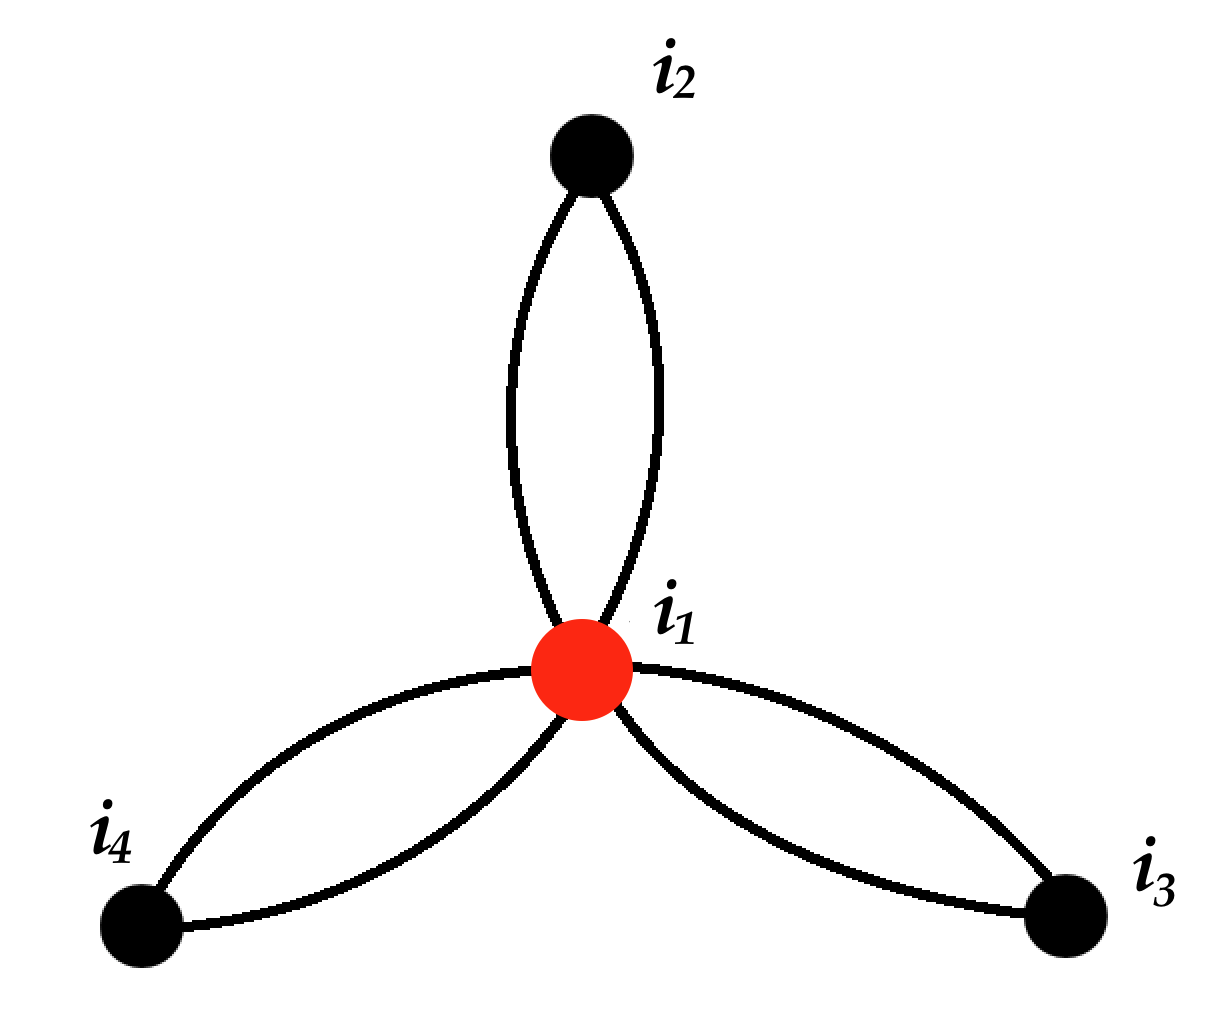
\includegraphics[scale = 0.15]{exemple-1.png}}
			\only<4>{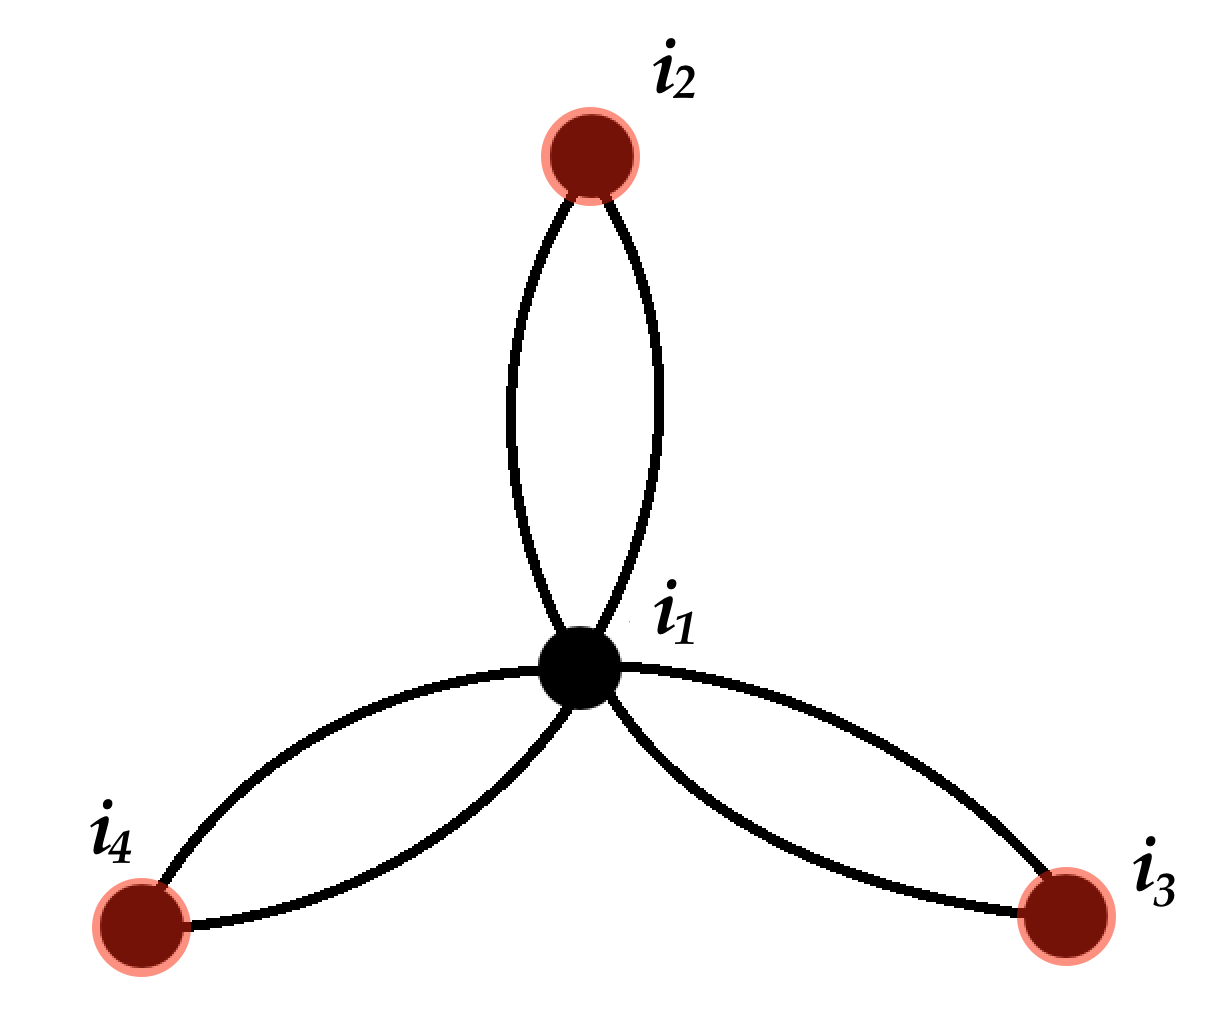
\includegraphics[scale = 0.15]{exemple-2.png}}

		\end{column}
	\end{columns}

\end{frame}

\section{Distribucions estacionàries}

\begin{frame}
	\frametitle{Distribució estacionària}
	Com és el passeig per a temps grans? \pause

	\begin{block}{Definició}
		Una distribució és \emph{estacionària} si \( \P(V(t) = u) = \P(V(t - 1) = u) \) per tot \( u \in V(G) \).
	\end{block} \pause

	En termes de la matriu de transició, \[ P\vec{\pi} = \vec{\pi}. \] \pause
	Per tant
	\begin{equation*}
		\vec{\pi}(u) = \sum_{v \in V(G)}\frac{a(u,v)}{\gr(v)} \vec{\pi}(v).
	\end{equation*}

\end{frame}

\begin{frame}
	\frametitle{Existència i unicitat de distribucions estacionàries}
	\begin{theorem}
		Tot graf connex admet una única distribució estacionària.
	\end{theorem}
	\pause

	\begin{block}{Demostració}
		\( \vec{\pi} \) estacionària. Veurem que \( \vec{\pi}(u) \propto \gr{u} \). \pause Sigui \( u^\ast \) tal que \( \frac{\vec{\pi}(u^\ast)}{\gr(u^\ast)} \) és màxim: \pause 
		\begin{equation*}
			\vec{\pi}(u^\ast) = \sum_{v \in V(G)} \frac{a(u^\ast,v)}{\gr(v)} \vec{\pi}(v) \pause \leq \frac{\vec{\pi}(u^\ast)}{\gr(u^\ast)} \sum_{v \in V(G)} a(u^{\ast},v) \pause = \vec{\pi}(u^\ast)
		\end{equation*}
		Aleshores \[ \sum_{v \in V(G)} a(u^\ast,v) \frac{\vec{\pi}(v)}{\gr(v)}  = \sum_{v \in V(G)} a(u^\ast,v) \frac{\vec{\pi}(u^\ast)}{\gr(u^\ast)}. \]  
	\end{block}
\end{frame}

\begin{frame}
	\frametitle{Existència i unicitat de distribucions estacionàries}
	\begin{proof}
		Per tant \( \frac{\vec{\pi}(v)}{\gr(v)} = \frac{\vec{\pi}(u^\ast)}{\gr(u^\ast)} \) per tot \( v \) adjacent a \( u^\ast \). \pause
		Podem extendre l'argument a tots els vèrtexs de \( G \) fent servir que és connex. \pause

		Com que \( \vec{\pi}(u) \propto \gr(u) \) aleshores \( \vec{\pi}(u) = C\gr(u) \). \pause

		Aleshores
		\begin{equation*}
			\sum_{u \in V(G)} \vec{\pi}(u) = C \sum_{u \in V(G)} \gr(u) \pause \implies C = \frac{1}{\sum_{u \in V(G)} \gr(u)} = \frac{1}{2\abs{E(G)}}
		\end{equation*} \pause
		I per tant 
		\begin{equation*}
			\vec{\pi}(u) = \frac{\gr(u)}{2 \abs{E(G)}}
		\end{equation*}

	\end{proof}
\end{frame}

\begin{frame}
	\frametitle{Convergència a la distribució estacionària}
	\begin{theorem}
		Tota distribució de probabilitats en un graf connex no bipartit convergeix a la distribució estacionària. 
	\end{theorem}
	\pause
	\begin{block}{Demostració}
\( P \) és similar a una matriu simètrica:
\[ D^{-1/2}PD^{1/2} = D^{-1/2}AD^{-1/2}. \] \pause
Per tant diagonalitza. \pause
\( \vec{\pi} \) és l'únic vector propi de valor propi 1. Posem \[ \vec{p}_0 = \alpha_1 \vec{\pi} + \sum_k \alpha_k \vec{v}_k \]
\end{block}
\end{frame}

\begin{frame}
	\frametitle{Convergència a la distribució estacionària}
	\begin{proof}
		Es pot demostrar que \( \alpha_1 = 1 \). \pause Aleshores
		\begin{equation*}
			P^t \vec{p}_0 = \vec{\pi} + \sum_k \lambda_k^t \alpha_k \vec{v}_k. 
		\end{equation*} \pause
		Per qualsevol graf, \( \abs{\lambda_k} \leq 1 \) i per un graf no bipartit \( \lambda_k > -1 \). \pause Per tant 
		\begin{equation*}
			P^t \vec{p}_0 \xrightarrow{t \to \infty} \vec{\pi}.
		\end{equation*}
	\end{proof}
\end{frame}

\begin{frame}
\frametitle{Grafs bipartits}
Pels grafs bipartits la convergència no es dóna, tal i com hem vist a l'exemple al principi. \pause

\centering
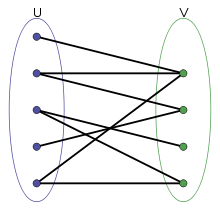
\includegraphics[scale = 0.7]{bipartit.png}
\end{frame}

\begin{frame}
\frametitle{Grafs bipartits}
Si permetem repetir vèrtexs aleshores obtenim un \emph{passeig aleatori mandrós}. \pause La matriu de transició és \[ \frac{1}{2}(I + P). \]
\end{frame}


\section{PageRank}
\begin{frame}
\frametitle{L'algorisme PageRank}
\begin{itemize}[<+->]
	\item Google desenvolupa un algoritme per determinar la rellevància de pàgines web. 
	\item Considera el graf dirigit dels híperenllaços entre pàgines i assigna a cada pàgina la probabilitat que li correspon a la distribució estacionària.  
	\item Per garantir la convergència es fan servir passejos mandrosos. 
	\item Com que el passeig és dirigit ja no tenim l'expressió de la distribució estacionària per a grafs no dirigits.
\end{itemize}
\end{frame}

\begin{frame}
\frametitle{Probabilitat de teletransport}
El caminant es teletransporta a un vèrtex aleatori amb probabilitat \( \alpha \). \pause 
\begin{equation*}
	P_\text{PR} = \frac{\alpha}{\abs{V(G)}}\bm{1} + \frac{1 - \alpha}{2}(I + P).
\end{equation*} \pause

A PageRank personalitzat ens trasalladem a un vèrtex concret: obtenim un rànquin relatiu a aquell vèrtex. \pause En general podem teletransportar-nos seguint una distribució qualsevol i obtindrem resultats rellevants a aquesta. 

\end{frame}

\section{El teorema de Pólya}
\begin{frame}
	\frametitle{Grafs infinits}
	Podem considerar passejos a grafs infinits. L'exemple més senzill són passejos aleatoris a \( \Z^d \)

	\centering
	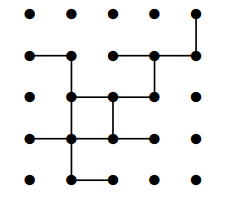
\includegraphics[width=50mm]{reticle.png}
\end{frame}

\begin{frame}
	\frametitle{Passejos recurrents i transitoris}
	\begin{block}{Definició}
		Anomenarem \emph{probabilitat d'escapament}, $p_\text{esc}$, a la probabilitat que el passeig aleatori mai retorni a l'origen.
	\end{block} \pause
	\begin{block}{Definició}
		Un passeig aleatori és \emph{recurrent} si i només si $p_\text{esc}=0$. 
		Un passeig aleatori és \emph{transitori} si i només si $p_\text{esc}>0$.
	\end{block}
\end{frame}

\begin{frame}
	\frametitle{Teorema de Pólya}
	\begin{theorem}
		Un passeig aleatori simple en una xarxa d-dimensional $\mathbb{Z}^d$ és recurrent si $d=1$ o $d=2$, i transitori si $d\geq 3$.
	\end{theorem} \pause

	\begin{block}{ }
		"A drunk man will find his way home, but a drunk bird may get lost forever." \\
		\textit{Shizuo Kakutani}
	\end{block}
\end{frame}
\end{document}
